\chapter{Módulo 4: Preparación}

Si tiene instalado el microcontrolador y el UNL2803, removerlos de sus zócalo antes de proseguir.

\section{Paso 1:}

Instalar pines hembras P4 (Pines para señal de entrada analógica)

\begin{figure}[h]
	\centering
	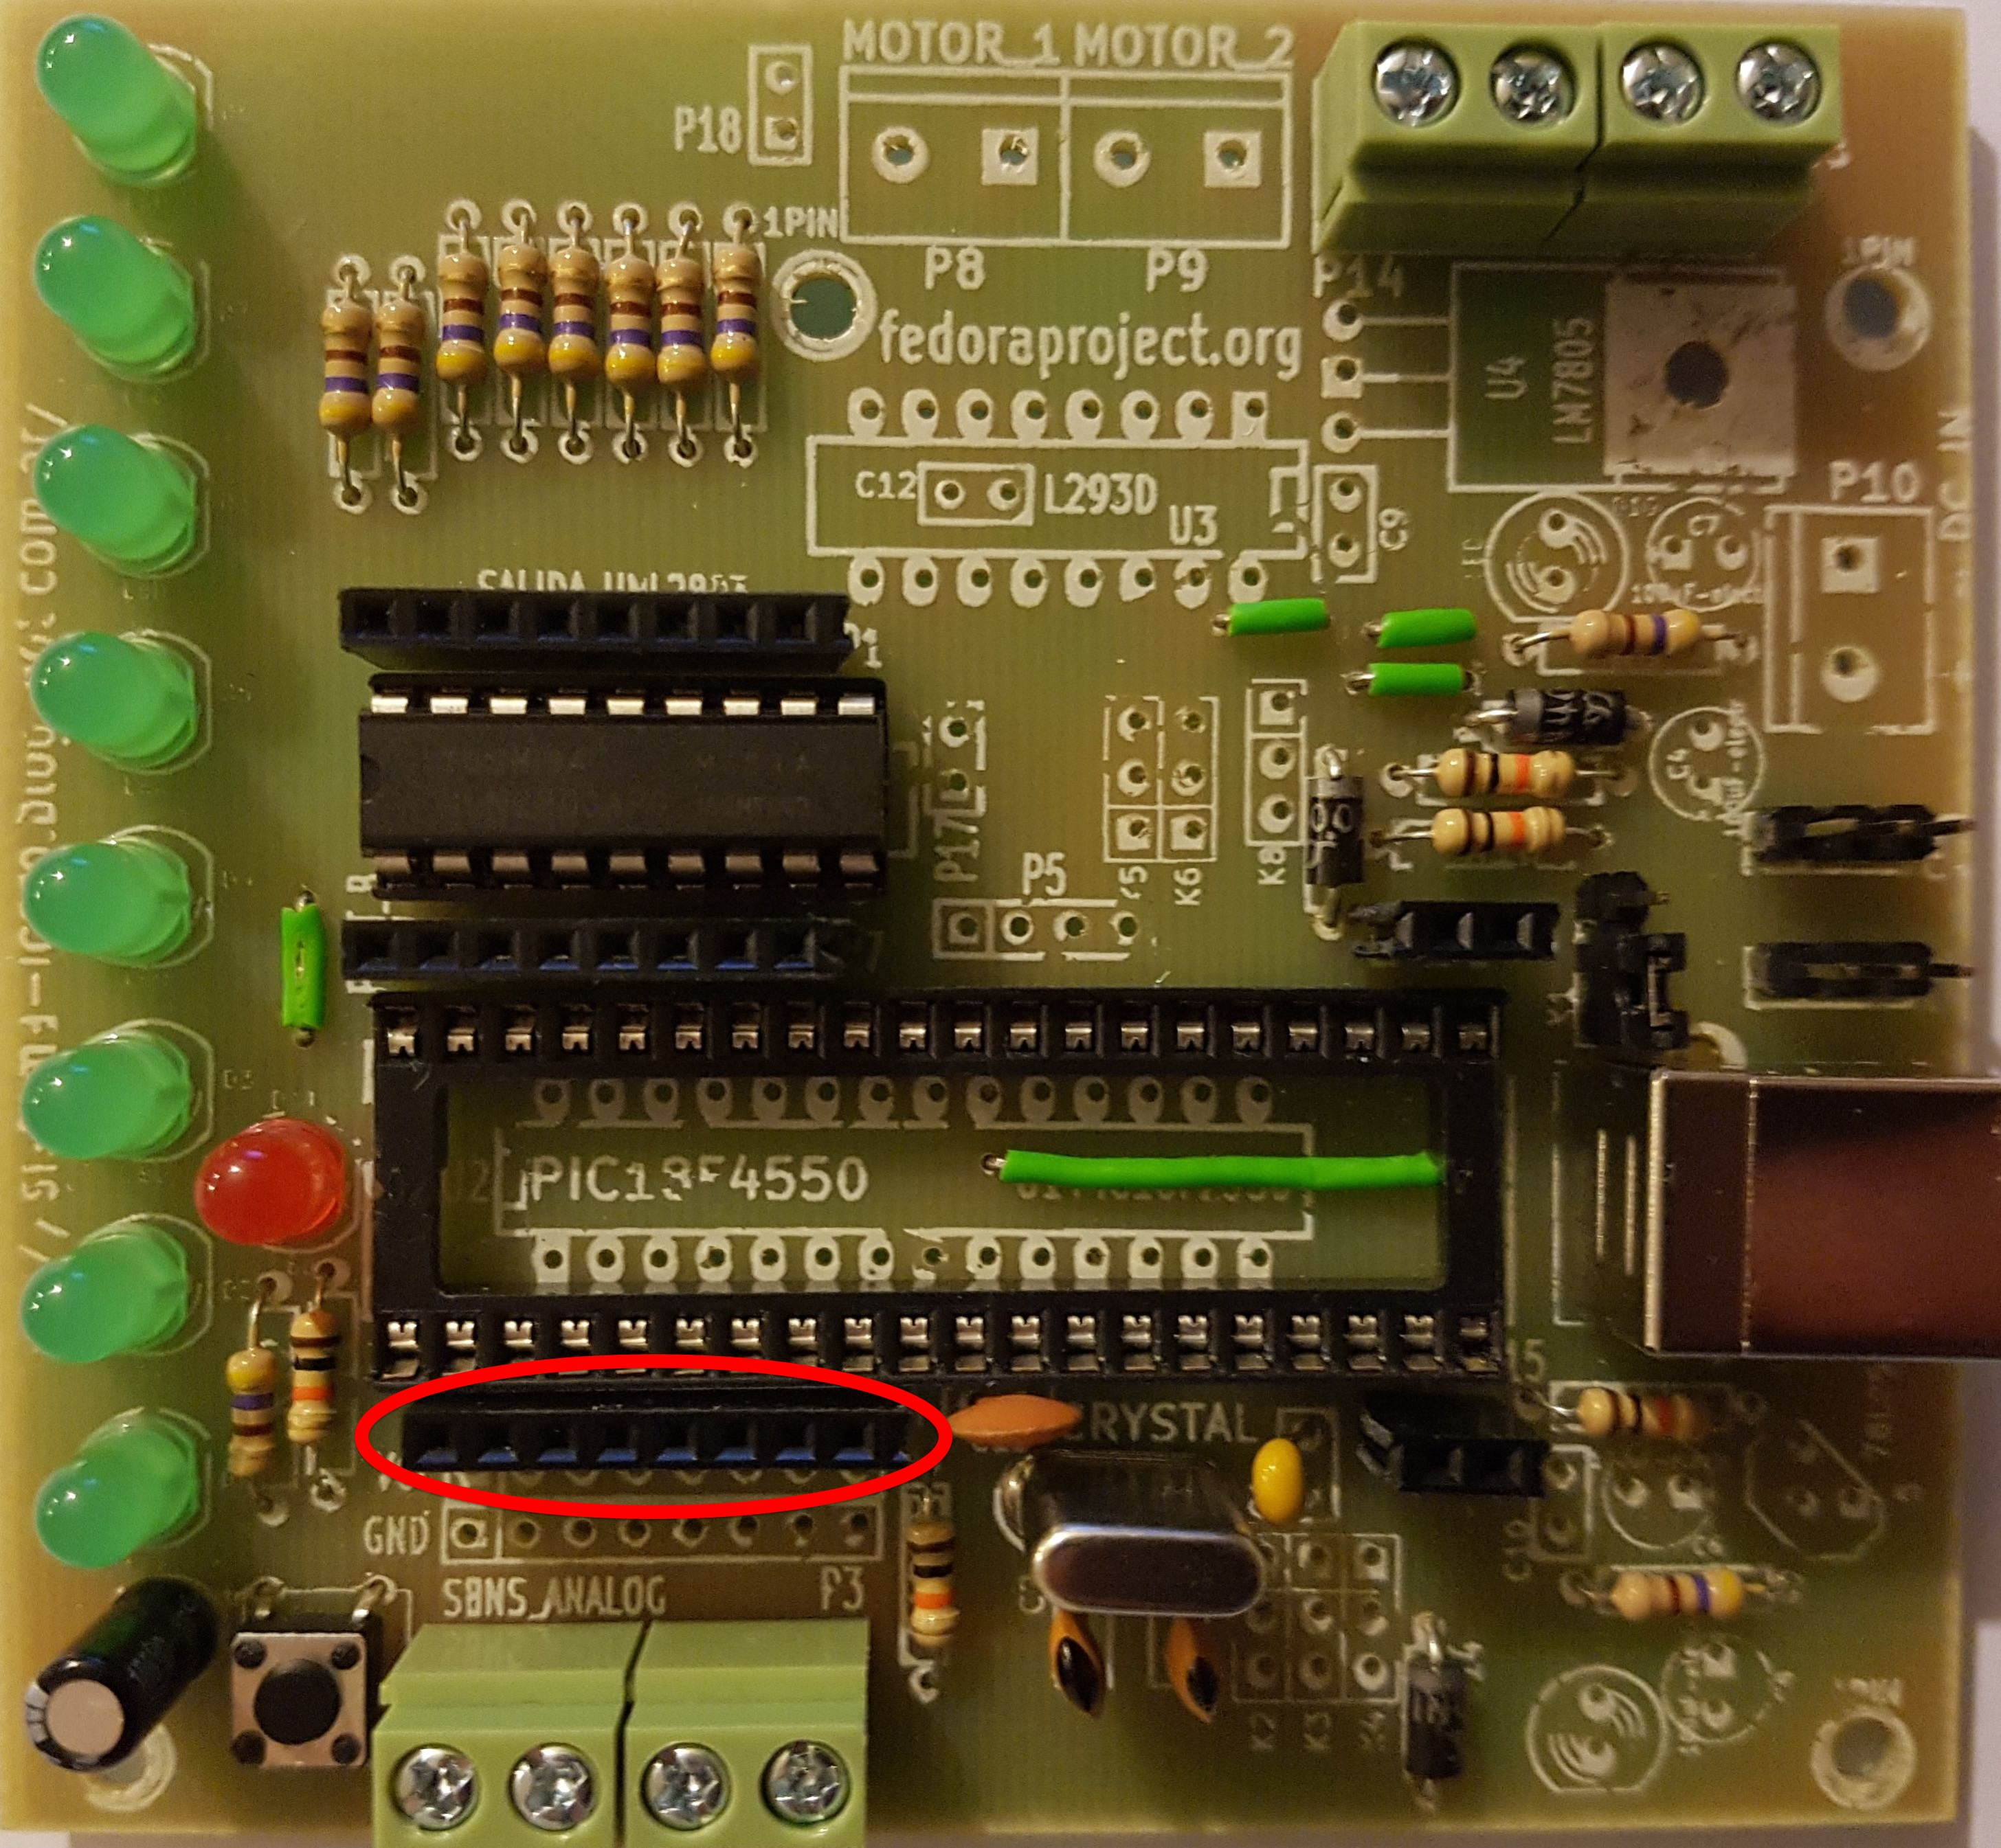
\includegraphics[width=0.8\linewidth]{Modulo_4/M4_1}
	\caption{Módulo 4 - Paso 1}
	\label{fig:M4_1}
\end{figure}

\newpage

\section{Paso 2:}

Instalar tira de pines hembras VCC. P2

\begin{figure}[h]
	\centering
	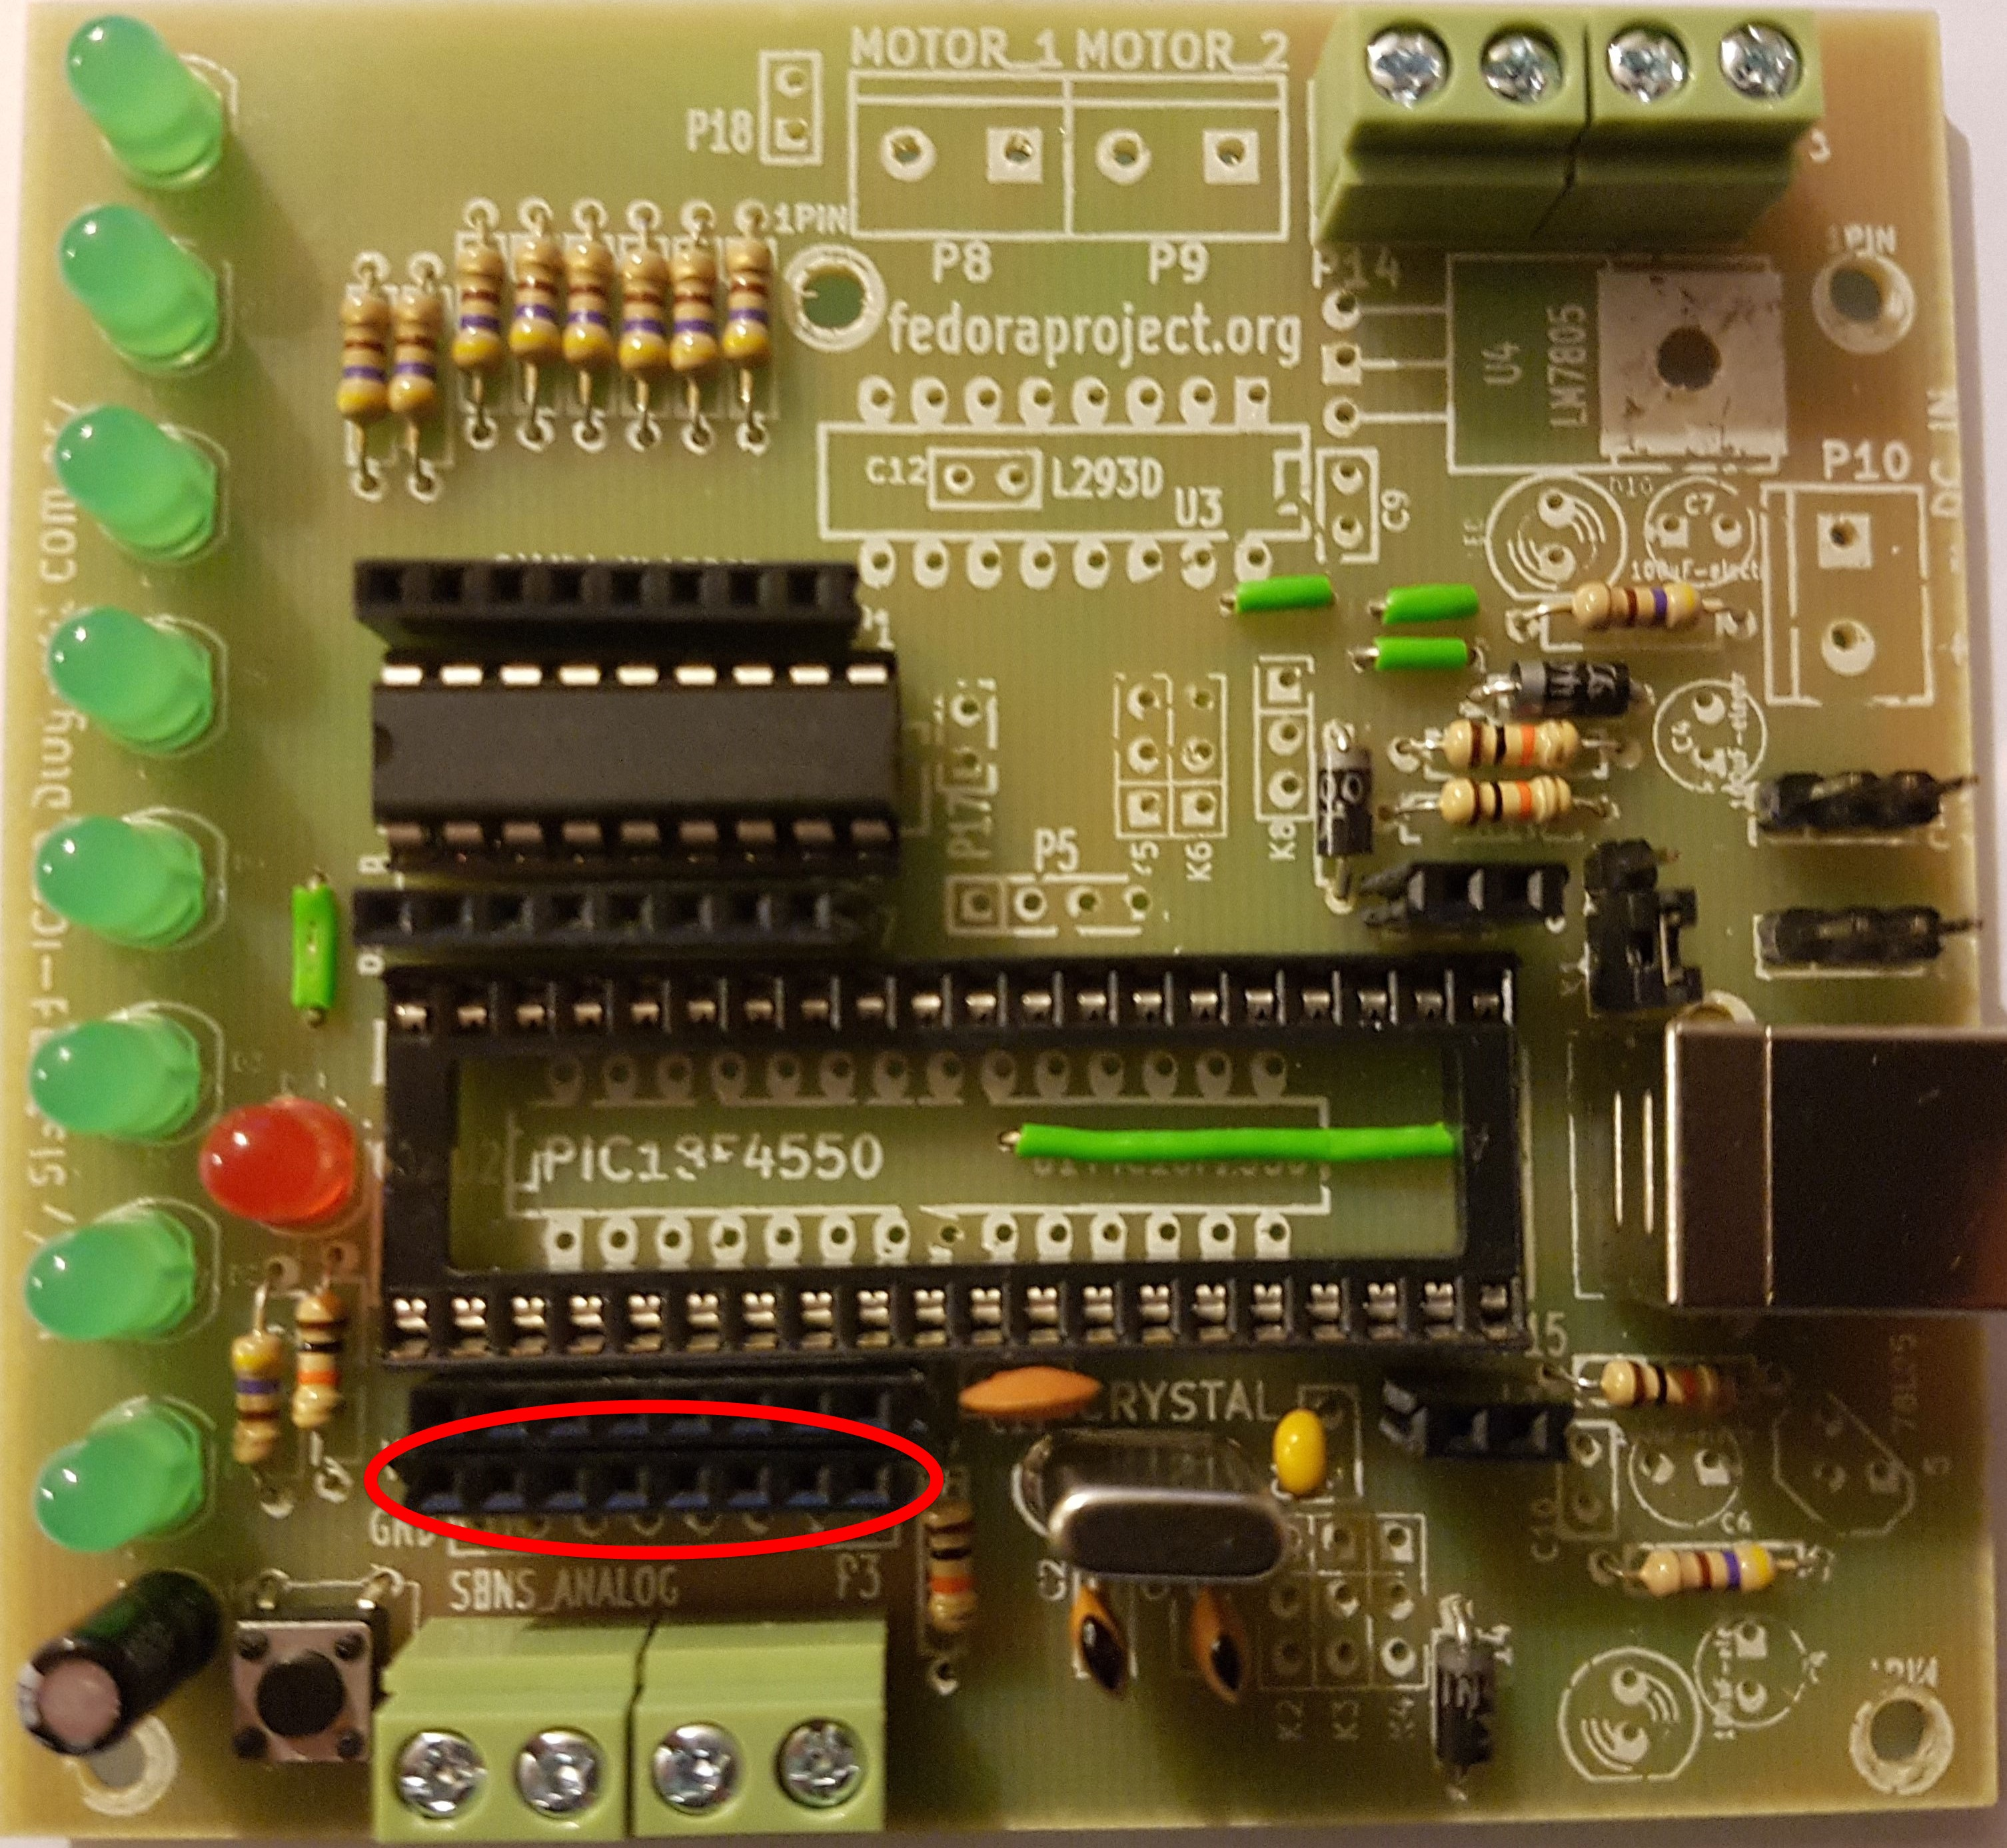
\includegraphics[width=0.8\linewidth]{Modulo_4/M4_2}
	\caption{Módulo 4 - Paso 2}
	\label{fig:M4_2}
\end{figure}

\newpage

\section{Paso 3:}

Instalar tira de pines hembras GND. P3

\begin{figure}[h]
	\centering
	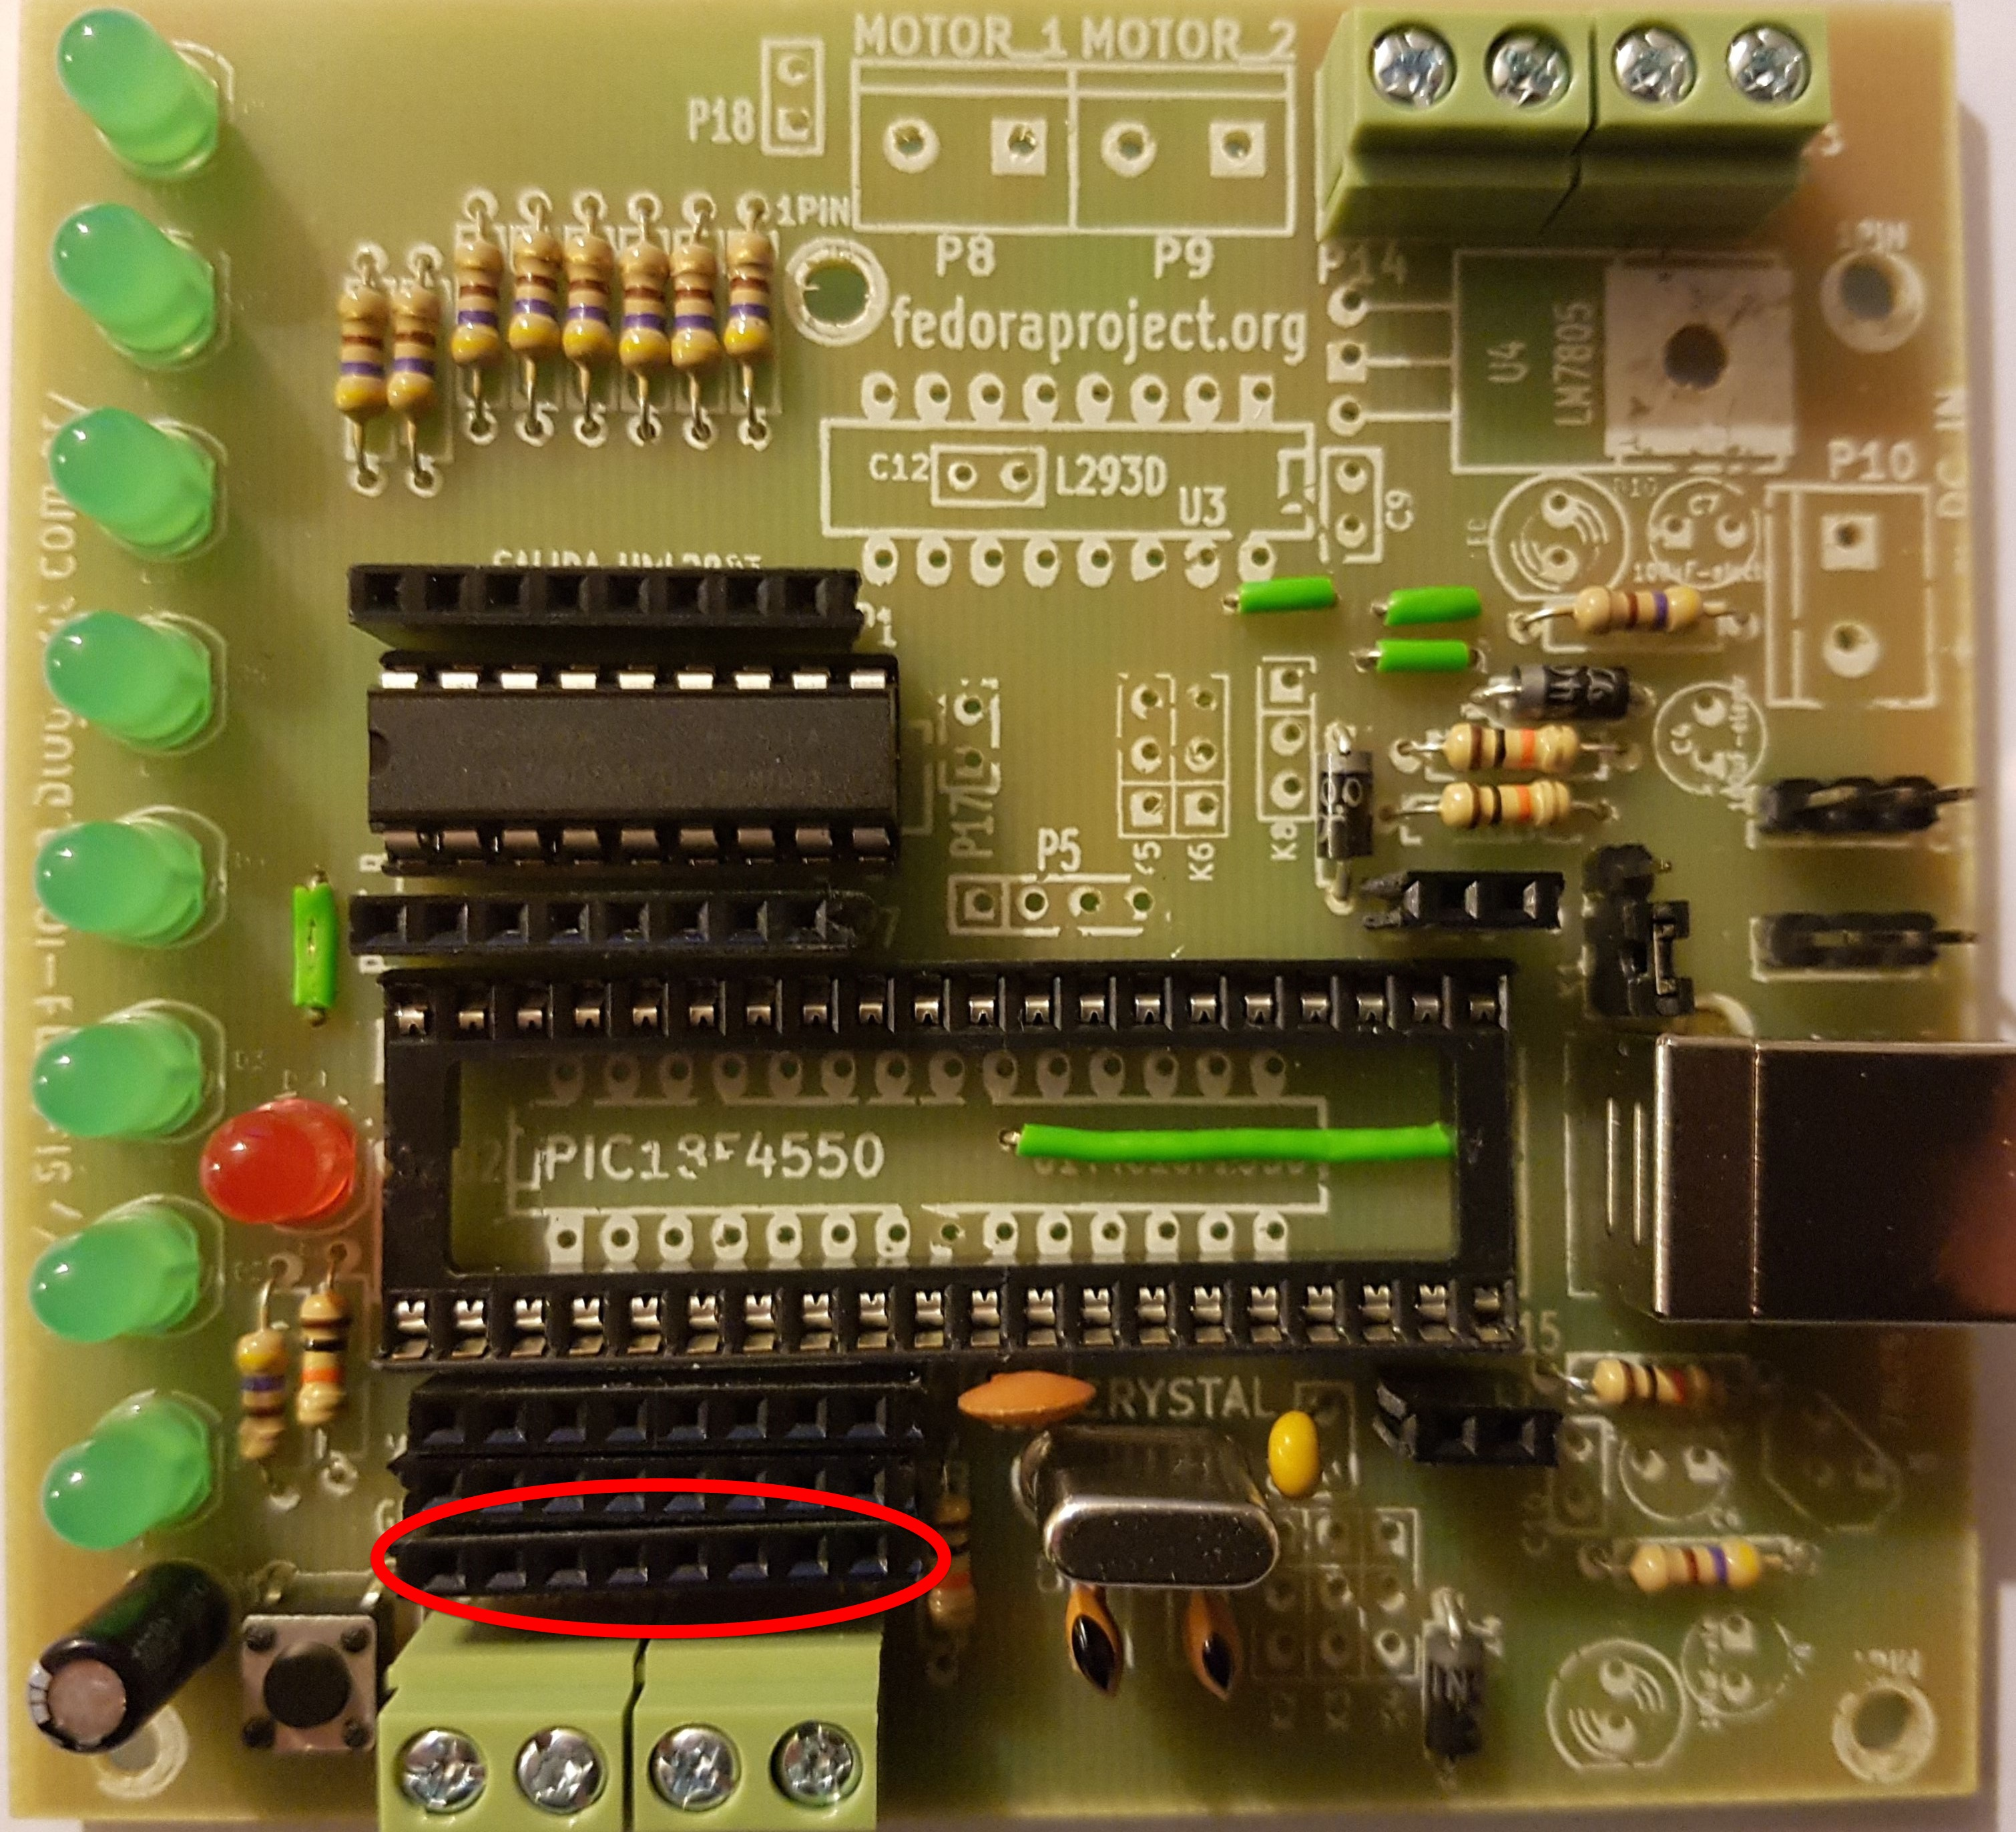
\includegraphics[width=0.8\linewidth]{Modulo_4/M4_3}
	\caption{Módulo 4 - Paso 3}
	\label{fig:M4_3}
\end{figure}

\newpage

\section{Paso 4:}

Instalar tira de pines machos de servos. K2 a K6

\begin{figure}[h]
	\centering
	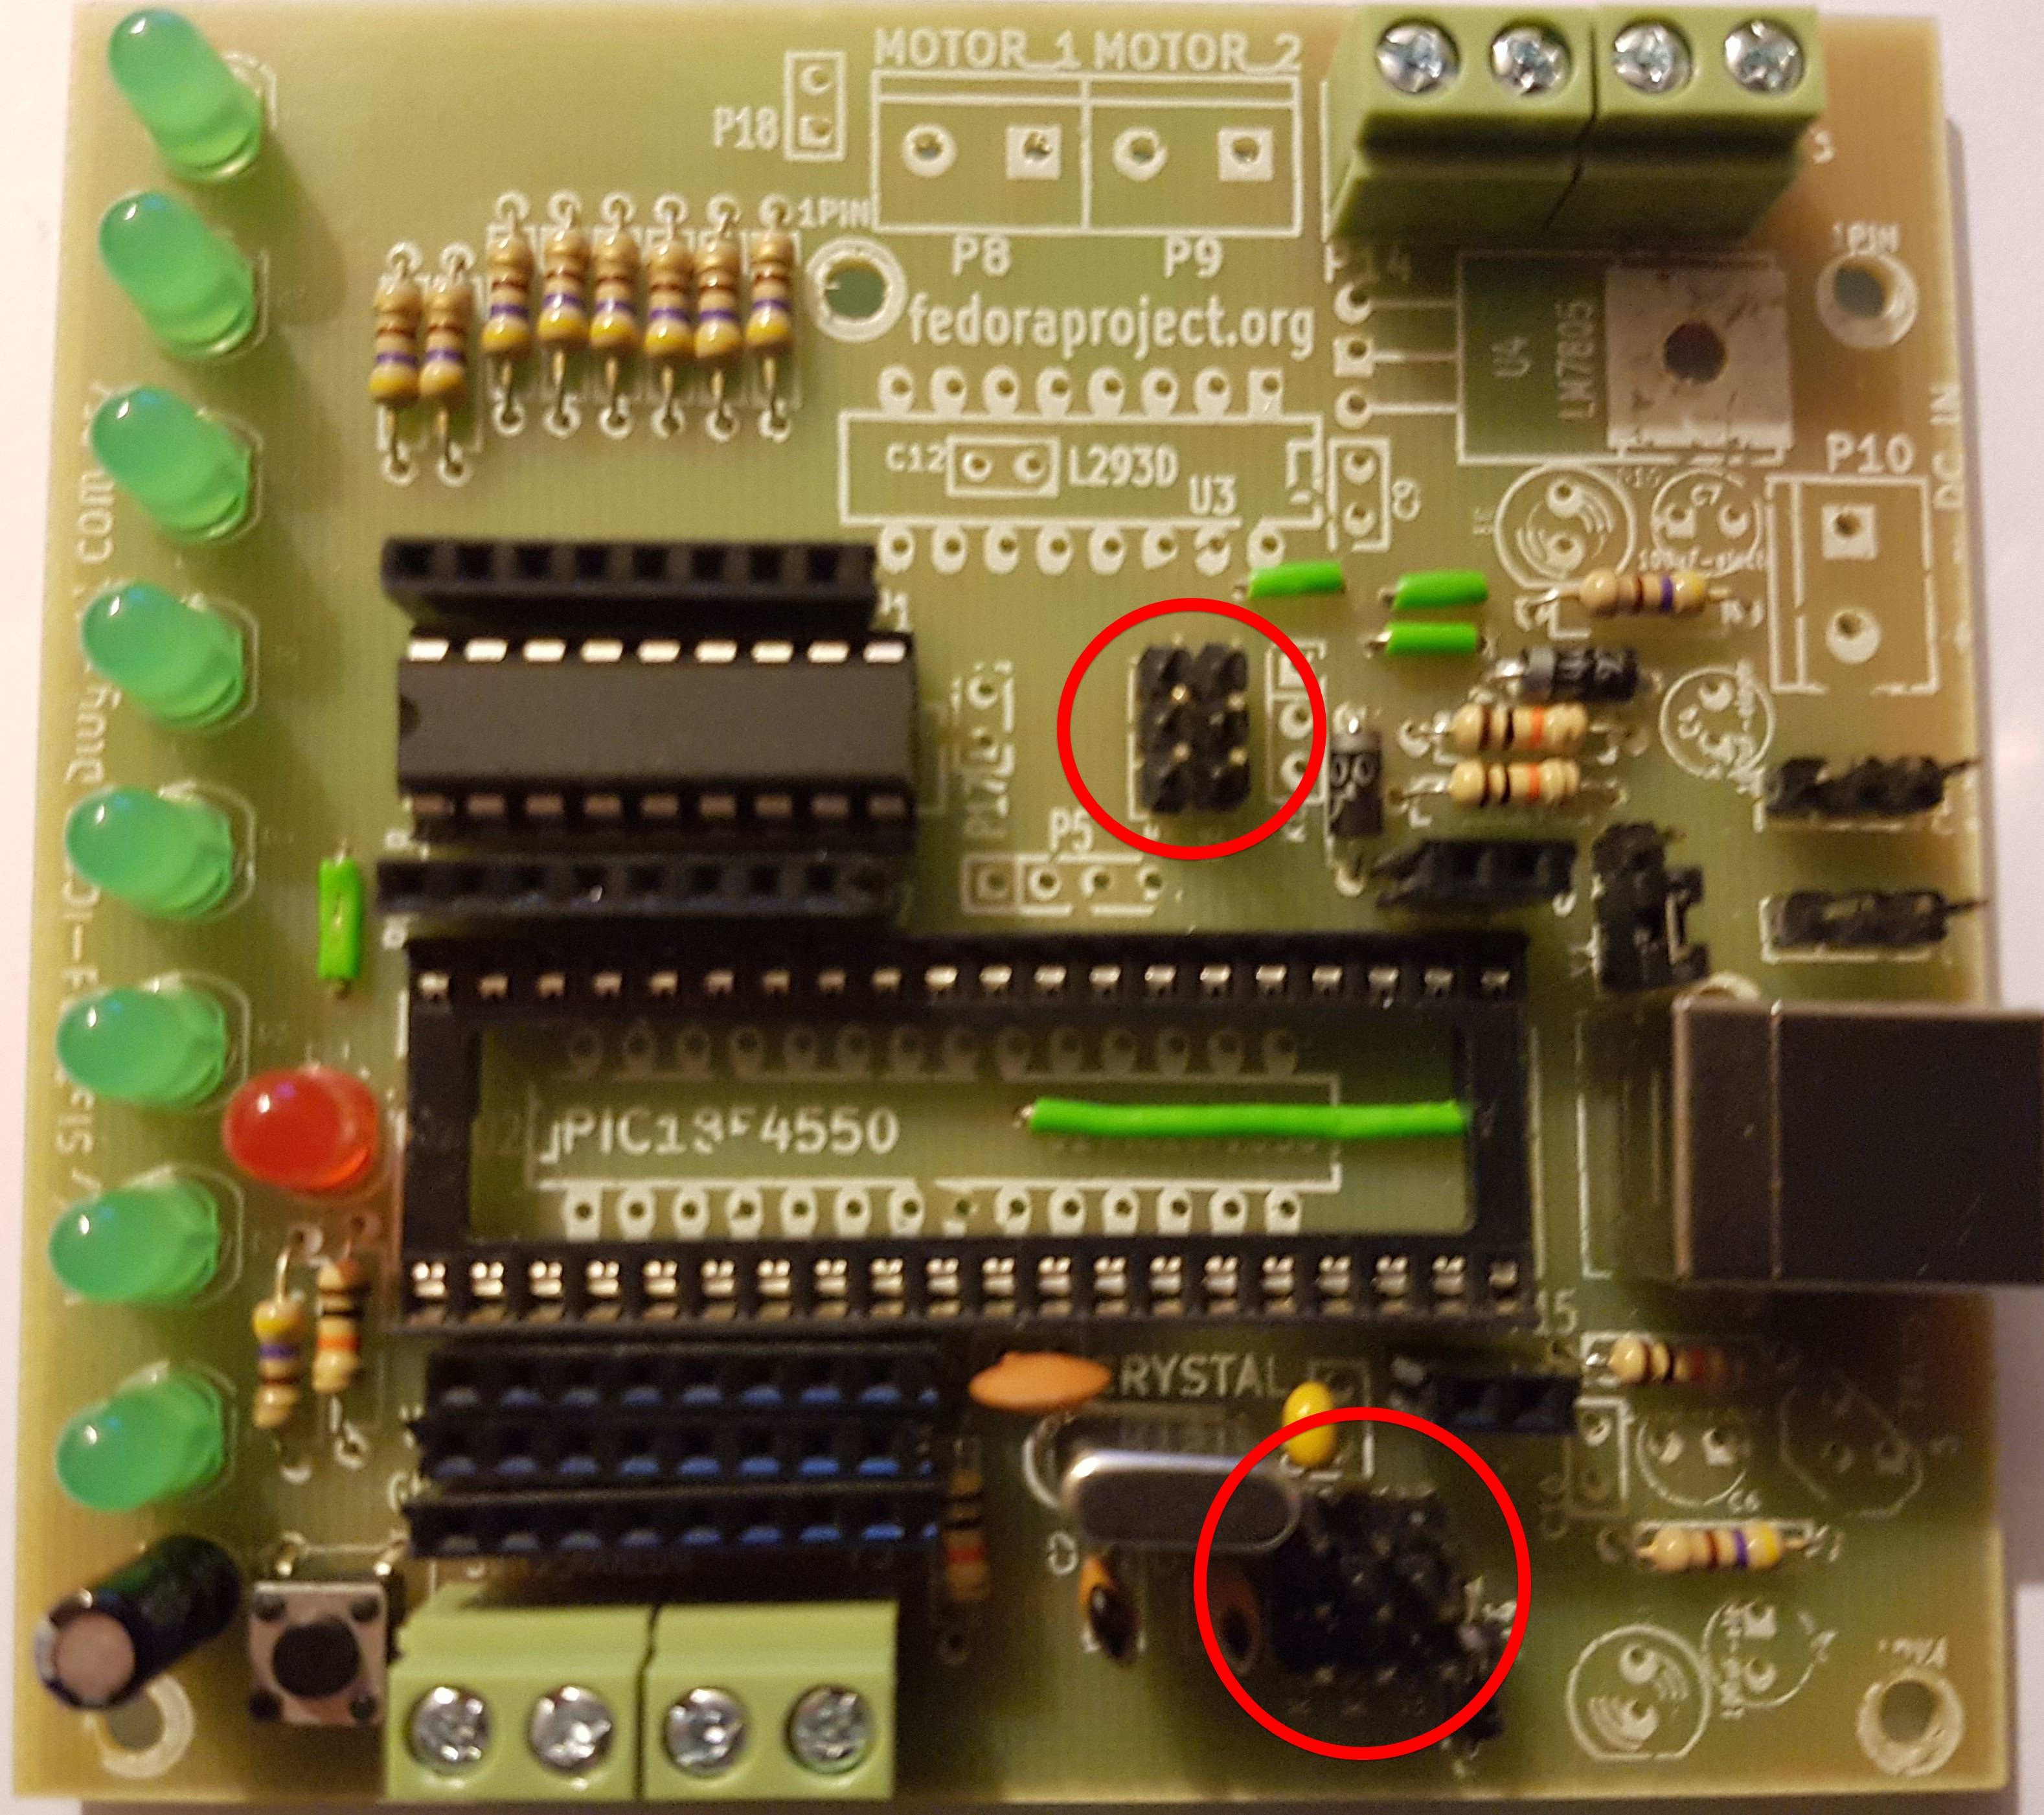
\includegraphics[width=0.8\linewidth]{Modulo_4/M4_4}
	\caption{Módulo 4 - Paso 4}
	\label{fig:M4_4}
\end{figure}

\newpage

Comprobación:
Cargar un script de ejemplos de la sección de icaro testing, sensors analogicos. Debe encenderse el led D8 y luego varios led aleatorios. Luego el led D7 y luego varios led aleatorios. Asi con cada uno de los leds. Los leds aleatorios son el valor de ruido que recibe el sensor analogico.

